\part{L'Intelligence Artificelle remplace l'humain pour les tâches répétitives}
\chapter{L'Intelligence Artificelle aujourd'hui}
L'intelligence Artificelle est un domaine faisant partie 
des sciences cognitives dont l'objectif est de mettre au
point des techniques et technologies permettant aux 
machines de simuler l'intelligence humaine ou animale.
Nous pouvons séparer l'IA en deux catégorie distinctes. 

\section{Intelligence Artificielle Faible}
Elle reproduit un comportement de manière le plus précise possible,
en s'ameliorant notamment grâce à l'apprentissage 
mais n'en n'imite pas le fonctionnement ce qui fait que
ce type d'IA ne fait que simuler de l'intelligence. \newline
Aujourd'hui il n'existe que des intelligences artificelles faibles qui peuvent  
être séparées en plusieurs technique et sous-domaines: \newline

\begin{figure}[H]
    \centering
    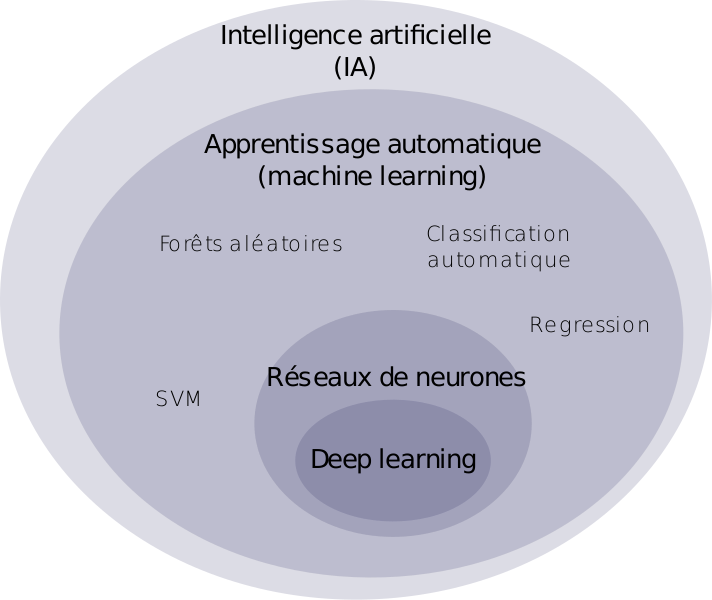
\includegraphics[width=0.8\textwidth]{Images/aitype}
    \caption{Les différents domaines de l'Intelligence Artificielle}
	\label{fig:DiffDomaineIA}
\end{figure}
\newpage

\subsection{Machine Learning}
Le Machine Learning est un ensemble de techniques qui permettent à un ordinateur 
d'agir et d'apprendre comme un humain tout en s'améliorant au fur et 
à mesure et ce de manière autonome. \newline

Le fonctionnement du machine learning ce découpe en plusieurs parties,
tout d'abord il faut définir des features, c'est à dire des
propriétés mesurables individuellement, cette partie est difficile et cruciale
car elle va déterminer l'efficacité de l'algorithme de machine learning. \newline

%je ne suis pas sur pour cette partie
Différents algorithme vont ensuite servir à extraire les features de données 
brut en entrée avant de les envoyer a l'algorithme de machine learning, par exemple 
la reconnaissance de bords ou de forme geométriques extraient les features d'une 
image dans une IA de reconnaissance d'image. \newline 

Enfin l'algorithme de machine learning va passer au travers de 3 sets de données:
\begin{itemize}
    \item un set de training va permettre d'entrainer l'algorithme de manière
     supervisé, ce set utilise des vecteurs d'entrée et leur sortie attendue.
    \item un set de validation qui va verifier le modèle crée à partir du set de 
    training.
    \item un set de test qui permet de tester la version finale de l'algorithme. 
    \newline
\end{itemize}

Le machine learning utilise les "réseaux de neurones", qui ont fait leurs premières 
apparition à partir de 1980, il s'agit de structure algorithmique imitant 
le comportement des neurones dans le cerveau humain:


\begin{figure}[H]
    \centering
    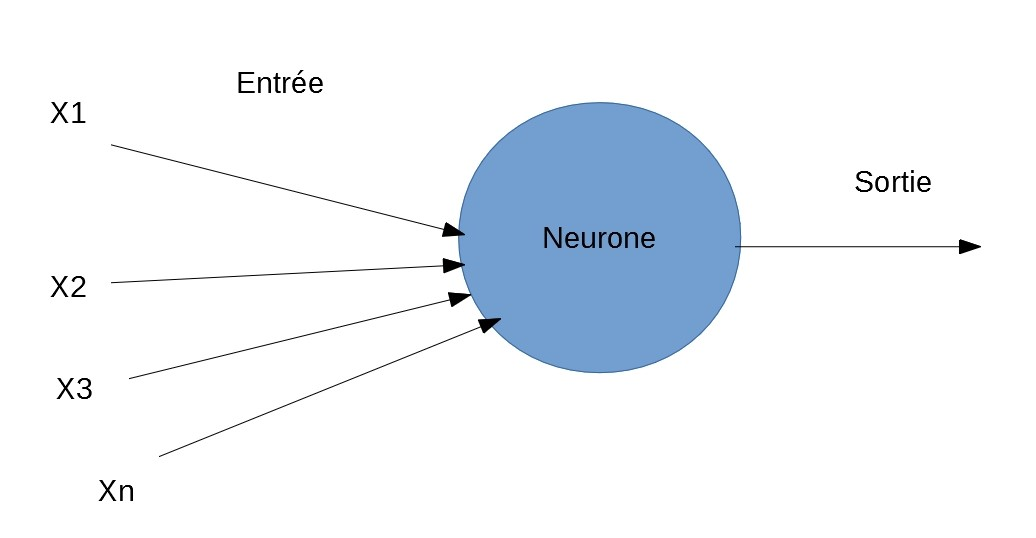
\includegraphics[width=0.6\textwidth]{Images/neuroneartificiel}
    \caption{Neurone Artificel}
	\label{fig:NN2Layers}
\end{figure}

Un neurone artificel comme son nom l'indique imite la topologie d'un neurone biologique,
ses entrées sont comparables aux dendrites d'un neurone tandis que sa 
sortie est l'équivalent de l'axone. \newline

les neurones sont divisé en différentes couches: couche d'entrée, couche(s) cachée
et couche de sortie, dans le cas du "shallow" machine learning, le réseaux de neurones 
n'est composé que d'une seule couche cachée: 

\begin{figure}[H]
    \centering
    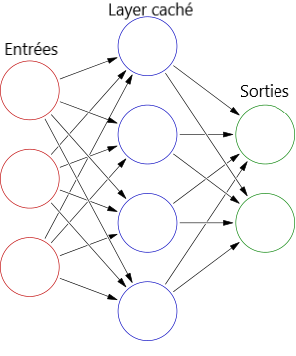
\includegraphics[width=0.4\textwidth]{Images/shallownnoverview}
    \caption{Réseau de neurones avec 2 couches cachées}
	\label{fig:NN2Layers}
\end{figure}

Ce type de réseaux de neurones est entrainé de manière supervisé mais dès lors qu'il 
y a plus d'une couche cachée, il n'est plus possible de l'entrainer ainsi,
l'alternative qui répond à ce problème est l'apprentissage profond ou 
deep learning qui utilise des réseaux de neurones avec de multiple couches 
cachées.  


\subsection{Deep Learning}
Le Deep Learning est une sous catégorie du machine learning qui s'est démocratisé
qu'à partir de 2010 et est une évolution des anciennes techniques de machine learning, 
la différence majeur réside dans le fonctionnement du traitement des 
informations, le machine learning traditionnel ou "shallow", en contraste avec le deep 
learning, réside dans la nécessité de selectionner manuellement les features 
qui doivent être identifiés par l'algorithme de machine learning:

\begin{figure}[H]
    \centering
    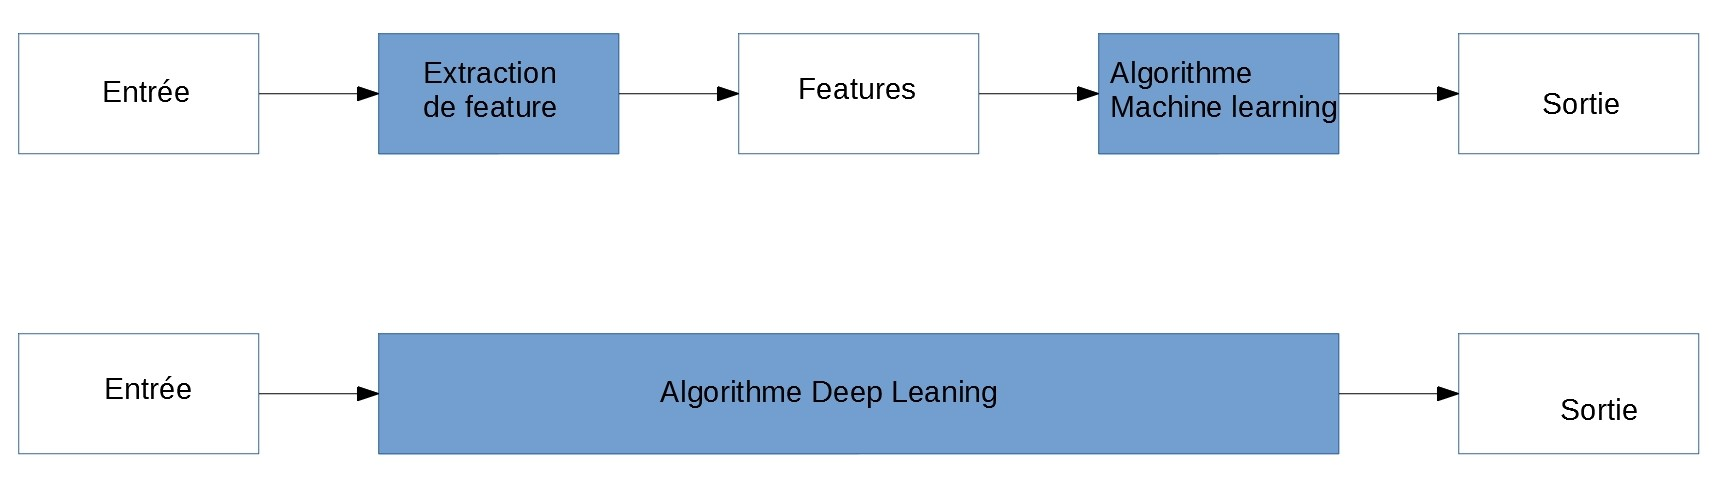
\includegraphics[width=1\textwidth]{Images/MLvsDL}
    \caption{Différences entre machine learning et deep learning}
	\label{fig:DiffMLDL}
\end{figure}

Le deep learning contrairement au machine learning n'a pas besoin de selectionner 
ou extraire manuellement les features, le modèle apprend par lui même à reconnaître 
des features, les réseaux de neurones utilisés pour le deep learning 
ont plus d'une couche caché de neurones d'où le nom "deep": \newline

\begin{figure}[H]
    \centering
    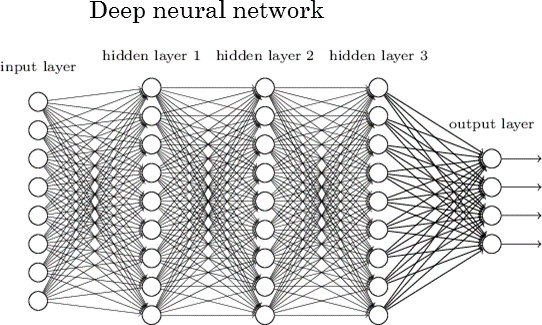
\includegraphics[width=0.7\textwidth]{Images/deepnn}
    \caption{Réseaux de neurones à 3 couches cachées}
	\label{fig:deepneuralnetwork}
\end{figure}

Ce qui fait la puissance du Deep Learning est sa capacité à avoir des Répresentations
intermediaires d'un niveau d'abstraction faible à un niveau d'abstraction élevé:

\begin{figure}[H]
    \centering
    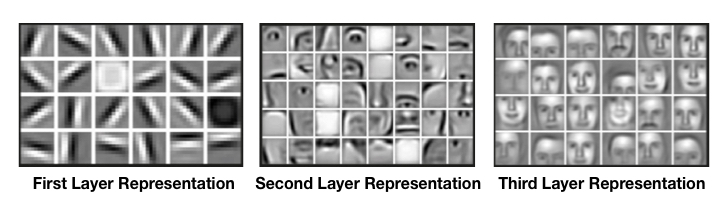
\includegraphics[width=1\textwidth]{Images/layeredrepresentation}
    \caption{Répresentations intermediaires - Andrew Ng}
	\label{fig:deepnnrepresentation}
\end{figure}

c'est celles-ci qui permettent de ne pas avoir à définir manuellement les features, 
dans l'exemple ci-dessus, l'algorithme extrait des features bas niveau dans la 
premières Répresentations, puis les assemble pour former des parties des 
visages puis finir par avoir des Répresentations de features de plus 
haut niveau donc des visages entier. \newline


\chapter{Applications de l'Intelligence Artificelle}
\section{Finance}
\section{Medicine}

